% numerical.tex

\cleardoublepage
\chapter{Optimised Ascent Trajectory}\label{chapter:Ascent}

\textcolor{red}{sensitivity study including: potentially max heating rate? max q, L/d (potentially varied viscous drag? as this is uncertain and has a magnitude change on the return trajectory), Isp, third stage mass and L/D}



This chapter presents a maximum payload-to-orbit trajectory optimisation for the rocket-scramjet-rocket launch system incorporating the SPARTAN. 
This chapter consists of a modified form of the Journal of Spacecraft and Rockets paper 'Trajectory Design of a Rocket-Scramjet-Rocket Multi-Stage Launch System' (accepted for publication). 
A constant dynamic pressure case with the minimum pull-up necessary for the third stage to achieve orbit is computed as a reference. The trajectory of the SPARTAN and third stage are optimised for maximum payload-to-orbit, and compared to the minimum pull-up trajectory. A sensitivity study is carried out by varying the maximum allowable dynamic pressure by $\pm$10$^\circ$, followed by increasing the drag by 10$^\circ$, and computing new optimal trajectory results. 



This chapter will be expanded to include a more thorough sensitivity analysis, including the variation of specific impulse, along with more data points for each parameter variation. The discussion on the sensitivity analysis will be refocussed to highlight the particular design attributes which may lead to performance variations.
Additionally the validation of each case will be discussed in detail, with forward simulation comparisons and optimality condition validations provided in appendices. 






\section{Current Methodology}

This section presents the current optimisation methodology, used to generate the optimised ascent trajectory results. This section will be updated to show the combined optimisation, and some details will be moved to Chapter 4. 



\subsubsection{Second Stage Optimisation - Constant Dynamic Pressure, Minimum Pull-Up}


The constant dynamic pressure case with minimum pull-up optimises the trajectory to minimise variation from the desired dynamic pressure, with the third stage release angle constrained to 1.5$^\circ$, approximately the minimum release angle necessary to reach orbit. This constraint results in a trajectory with the smallest possible pull-up manoeuvre. 
The trajectory is configured with a quadratic cost function centred around 50kPa dynamic pressure:
\begin{equation} 
\min\limits_{\textbf{u}_2} \quad C_2(\textbf{x}_{2}(t_2),\textbf{u}_{2}(t_2))
\end{equation}
where
\begin{equation}
C_2(\textbf{x}_{2}(t_2),\textbf{u}_{2}(t_2)) = \int_{t_{2,0}}^{t_{2,f}} \frac{(\textit{\textbf{q}}-50\times 10^3)^2+10^5}{10^5} \, dt
\end{equation}
This quadratic function provides a smooth, continuous function to increase solver stability and ensure uniform dynamic pressure. Scaling and translating constants of $10^5$ are included to normalize the cost function, in order to improve the accuracy and stability of the solution. Second-third stage separation occurs when the scramjet has expended all of its fuel.  The third stage is then optimised for maximum payload from the calculated second-third stage separation point. 

In order to ensure an optimal solution, the number of nodes which DIDO uses is manually varied between 96-105, and a solution computed for each node value to ensure a distinct local minima. Ten solutions is observed to provide a sufficient number of node variation, with the solutions converging to similar local minima. The range of node values is chosen to produce accurate solutions, with efficient computation times. The final solution chosen corresponds to the node value which most minimises the cost function, and thus minimises the deviation from the 50kPa dynamic pressure trajectory. 

\subsubsection{Second Stage Optimisation - Maximised Payload}
For the maximum payload optimisation, the second and third stages are considered using a dynamic programming approach. First, in order to increase the computational efficiency of the optimisation, optimal third stage payloads are tabulated  over a 3 degree grid of separation conditions, $\textbf{x}_2(t_{2,f})$, as described in Section \ref{section:thirdstage}, providing the optimal payload for a range of velocity, altitude and flight path angles at separation as shown in Figure \ref{fig:contours}. Then, the interpolated third stage payload is used as the terminal cost $C_{2 \rightarrow 3}(\textbf{x}_2(t_{2,f}))$ for the calculation of the second stage trajectory optimisation, which optimises both the second and third stages by setting the cost function to maximise payload:
\begin{equation}
\min\limits_{\textbf{u}_2} \quad C_2(\textbf{x}_{2}(t_2),\textbf{u}_{2}(t_2) + C_{2 \rightarrow 3}(\textbf{x}_2 (t_{2,f}))
\end{equation}
where
\begin{equation}
C_2(\textbf{x}_{2}(t_2),\textbf{u}_{2}(t_2)) = 0.01\int_{t_{2,0}}^{t_{2,f}}\dot{m}_{fuel} \, dt
\end{equation}
\begin{equation}
C_{2 \rightarrow 3}(\textbf{x}_2(t_{2,f})) = -m_{payload}.
\end{equation}
$C_{2}(\textbf{x}_{2}(t_2),\textbf{u}_{2}(t_2))$ is included to improve numerical stability and is weighted by a constant, 0.01, in order to have negligible effect on the resultant trajectory.
This problem is solved using the pseudospectral method\cite{Ross2004}.  As with the constant dynamic pressure case, the number of nodes is manually varied between 96-105, and a solution computed for each node value, converging to similar local minima. The final solution chosen corresponds to the node value which most maximises the payload-to-orbit of the vehicle.
The third stage is optimised for maximum payload from the calculated second-third stage separation point, as a check to ensure that the interpolation has provided an accurate payload-to-orbit result. 


\section{Optimised Ascent Trajectory Results}


LODESTAR is used to investigate the suitability of a pseudospectral method approach to optimisation of scramjet-rocket trajectories and to develop optimal trajectory solutions. The following trajectories are developed: 
\begin{enumerate}
	\item: $q = $ 50kPa fixed SPARTAN trajectory with minimum pull-up \newline$\rightarrow$ Verifies simulation and provides baseline trajectory.
	\item: Trajectory optimised for payload-to-orbit, $q_{max} = $ 50kPa \newline$\rightarrow$ Demonstrates improved performance through coupled trajectory optimisation.
	\item: Trajectory optimised for payload-to-orbit, $q_{max} = $ 45kPa \& $q_{max} = $ 55kPa \newline$\rightarrow$ Comparison of these simulations allows investigation into the effect of $q$ max on payload-to-orbit.
	\item: Trajectory optimised for payload-to-orbit,  $q_{max} = $ 50kpa, 110\% SPARTAN Drag \newline$\rightarrow$ Comparison of optimal trajectories at 100\% and 110\% drag allows investigation of the robustness of the solution with variation in vehicle design. 
\end{enumerate}

Table \ref{table:Summary} details key results for comparison. 


\begin{table}[htb]
	\centering
	\caption{Summary of Simulation Results}
	\small
	\begin{tabular}{l c c c c c}
		& \textbf{1} & \textbf{2} & \textbf{3a} & \textbf{3b} & \textbf{4}  \\ 
		
		
		
		\hline  \begin{tabular}{@{}c@{}} \textbf{Trajectory Condition}\\  \\  	\end{tabular} &  \begin{tabular}{@{}c@{}}\textbf{$q = $ 50kPa} \\\textbf{$\gamma_{2\rightarrow 3}$= 1.5$^\circ$}\end{tabular}&  \begin{tabular}{@{}c@{}}\textbf{$q \leq $ 50kPa} \\ \textbf{Max $m_{Payload}$}\end{tabular}& \begin{tabular}{@{}c@{}}\textbf{ $q \leq $ 45kPa}  \\ \textbf{Max $m_{Payload}$} \end{tabular} & \begin{tabular}{@{}c@{}}\textbf{$q \leq $ 55kPa} \\\textbf{Max $m_{Payload}$} \end{tabular} &  \begin{tabular}{@{}c@{}}\textbf{$q \leq $ 50kPa} \\ \textbf{Max $m_{Payload}$} \\ \textbf{110\% $C_D$} \end{tabular} \\ 
		
		
		
		\hline \textbf{Payload to Orbit (kg)}  & \PayloadToOrbitConstq & \PayloadToOrbitFiftykPa & \PayloadToOrbitFortyFivekPa & \PayloadToOrbitFiftyFivekPa & \PayloadToOrbitHighDrag \\ 
		\textbf{Separation Alt, 1$\rightarrow$2 (km)}  & \FirstStageAltConstq & \FirstStageAltFifty & \FirstStageAltFortyFive &  \FirstStageAltFiftyFive &\FirstStageAltHighDrag \\ 
		\textbf{1$^{st}$ Stage Structural Mass Fraction} & \FirstStagesmfConstq & \FirstStagesmfFifty &  \FirstStagesmfFortyFive& \FirstStagesmfFiftyFive  & \FirstStagesmfHighDrag\\ 
		\textbf{Separation Alt, 2$\rightarrow$3(km)}  & \SeparationAltConstq & \SeparationAltFiftykPa & \SeparationAltFortyFivekPa & \SeparationAltFiftyFivekPa & \SeparationAltHighDrag\\ 
		\textbf{Separation $v$, 2$\rightarrow$3(m/s)} & \SeparationvConstq  & \SeparationvFiftykPa & \SeparationvFortyFivekPa &  \SeparationvFiftyFivekPa & \SeparationvHighDrag\\ 
		\textbf{Separation $\gamma$, 2$\rightarrow$3(deg)} & \SeparationAngleConstq& \SeparationAngleFiftykPa &\SeparationAngleFortyFivekPa& \SeparationAngleFiftyFivekPa&\SeparationAngleHighDrag \\ 
		\textbf{Separation $q$, 2$\rightarrow$3(kPa)} & \SeparationqConstq  &\SeparationqFiftykPa&\SeparationqFortyFivekPa &\SeparationqFiftyFivekPa& \SeparationqHighDrag \\ 
		\textbf{2$^{nd}$ Stage L/D, 2$\rightarrow$3} & \SeparationLDConstq&\SeparationLDFiftykPa & \SeparationLDFortyFivekPa & \SeparationLDFiftyFivekPa &\SeparationLDHighDrag\\
		\textbf{2$^{nd}$ Stage Flight Time (s)} & \FlightTimeConstq & \FlightTimeFiftykPa & \FlightTimeFortyFivekPa & \FlightTimeFiftyFivekPa & \FlightTimeHighDrag\\ 
		%\textbf{3$^{rd}$ Stage Max $q$ (kPa)} &\MaxqConstq  &\MaxqFiftykPa & \MaxqFortyFivekPa &\MaxqFiftyFivekPa & \MaxqHighDrag\\ 
		\textbf{3$^{rd}$ Stage $t$, $q >$ 20kpa (s)} &\toverConstq &\toverFiftykPa &\toverFortyFivekPa &\toverFiftyFivekPa & \toverHighDrag\\ 
		
		
		\hline 
	\end{tabular} 
	
	
	\label{table:Summary}
\end{table}


\subsection{First Stage Evaluation - q=50kpa Second Stage Separation}

\begin{figure}[ht]
	\centering
	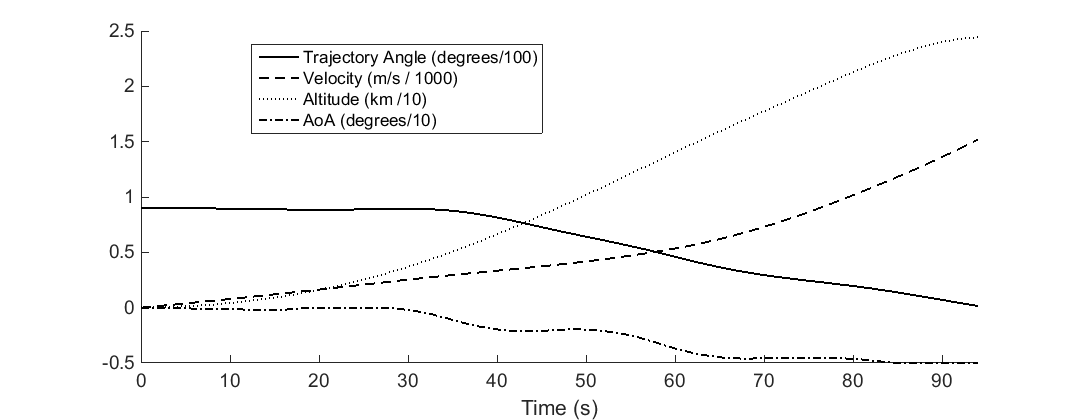
\includegraphics[width=.9\linewidth]{figures/5_Ascent/FirstStage}
	\caption{First stage trajectory, optimised for minimum fuel mass and a release point of 50kPa.}
	\label{fig:FirstStage}
\end{figure}



Figure \ref{fig:FirstStage} shows an example first stage trajectory, optimised for minimum mass, with end conditions of 24.4km altitude and 1.56$^\circ$ flight path angle. These separation conditions correspond to the second stage separation conditions for a 50kpa dynamic pressure trajectory.

The first stage flies a fixed vertical trajectory for 3.79s, after which a pitchover is initiated. 
After pitchover the angle of attack reduces to -1.17$^\circ$ at 13.1s. The angle of attack is then raised to 0.88$^\circ$ at 29.9s, before reducing gradually to the minimum of -5$^\circ$, adjusting in stages in order to reach the desired end conditions. 
An altitude of 24.4km is reached after a total flight time of 93.6s, with a total ground distance of 34.5km covered. 
This trajectory shape is very similar for all first stage simulation cases. 



\subsection{Second Stage Evaluation}
\subsubsection{Fixed Dynamic Pressure Trajectory, Minimum Pull-Up} \label{subsection:Fixed}

\begin{figure}[ht]
	\centering
	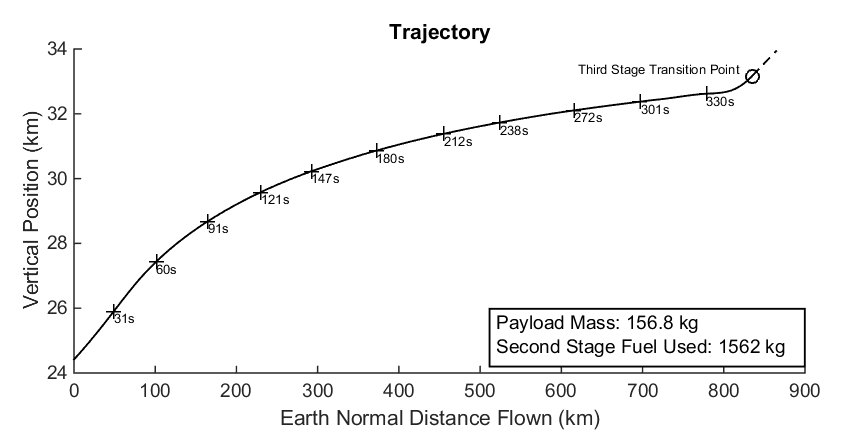
\includegraphics[width=.7\linewidth]{figures/5_Ascent/Constq}
	\caption{Trajectory path of the 2$^{nd}$ stage SPARTAN vehicle flying at 50kPa constant dynamic pressure, with 1.5$^\circ$ third stage release angle.}
	\label{fig:constq}
\end{figure}
\begin{figure}[ht]
	\centering	
	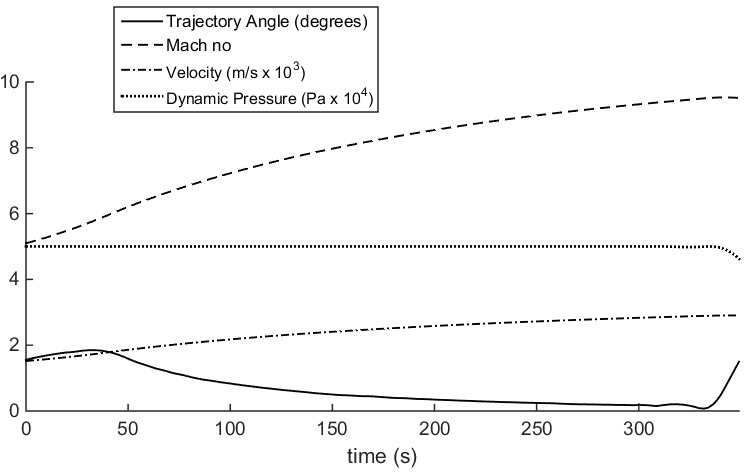
\includegraphics[width=.6\linewidth]{figures/5_Ascent/Constq-Aero}
	\caption{Trajectory data for 50kPa constant dynamic pressure trajectory, with 1.5$^\circ$ third stage release angle.}
	\label{fig:constq aero}
\end{figure}
\begin{figure}[ht]
	\centering
	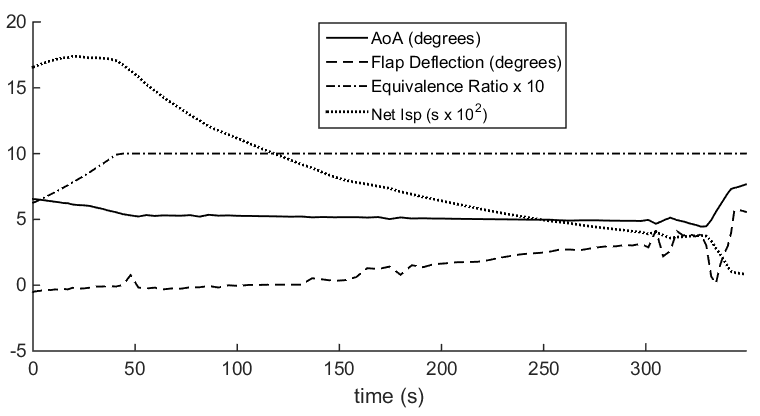
\includegraphics[width=.6\linewidth]{figures/5_Ascent/Constq-Vehicle}
	\caption{Vehicle performance data for 50kPa constant dynamic pressure trajectory, with 1.5$^\circ$ third stage release angle. Note: Flap deflection is positive down.}
	\label{fig:constq vehicle}
\end{figure}


A constant dynamic pressure trajectory with a pull-up to 1.5$^\circ$ flight path angle at third stage release is produced as a baseline for comparison with a payload-optimised trajectory, and to verify that LODESTAR is able to optimise a complex airbreathing trajectory. A pull-up to 1.5$^\circ$ flight path angle is the minimum necessary for the third stage to reach orbit. At release angles below 1.5$^\circ$, the thrust vector limitations necessary to produce a trimmed trajectory constrain the angle of attack of the third stage so that the rocket does not generate the lift required to exit the atmosphere. This angle of attack limitation, imposed by the maximum thrust vector, necessitates a scramjet-stage pull-up manoeuvre in order for the third stage rocket to operate successfully. 


The constant dynamic pressure, minimum pull-up trajectory for the SPARTAN stage is shown in Figures \ref{fig:constq}, \ref{fig:constq aero} and \ref{fig:constq vehicle} with key results summarised in Table \ref{table:Summary}. Due to the clear objective of a constant dynamic pressure trajectory, any deviations from the target dynamic pressure are readily apparent, allowing the efficacy of the optimiser to be verified. 
These results show very close adherence to 50kPa dynamic pressure (maximum 0.29\% deviation) until pull-up at 336.4s. Third stage release occurs at \FlightTimeConstq s at \SeparationAltConstq km altitude. 
Over the trajectory the Mach no. increases from 5.10 to 9.52 and the velocity from 1520m/s to \SeparationvConstq m/s. The flap deflection shows an overall increase from $-0.53^\circ$ to $5.76^\circ$ over the trajectory.  The net specific impulse ($I_{sp_{net}} = \frac{T-D}{\dot{m}_f g}$) generally decreases over the trajectory, as the efficiency of the scramjet engines decreases. However, at the beginning of the trajectory the equivalence ratio increases as the capture limitations are relaxed with increasing Mach number. This causes the net specific impulse to increase, to a maximum of 1739s, during the first 19.45s flight time. 

Figure \ref{fig:ThirdStageConstQ} shows the corresponding third stage atmospheric exit trajectory after release, evaluated as described in Chapter \ref{chapter:LODESTAR}. After atmospheric exit, this trajectory is followed by a Hohmann transfer to a heliosynchronous orbit, resulting in a total payload to orbit of \PayloadToOrbitConstq kg.



\subsubsection{Dynamic Pressure Limited Trajectory} \label{subsection:50kPalimit}



\begin{figure}[ht]
	\centering
	\includegraphics[width=.7\linewidth]{figures/5_Ascent/qlimited50kPa}
	\caption{Maximum payload trajectory path of the 2$^{nd}$ stage SPARTAN vehicle when limited to 50kPa dynamic pressure.}
	\label{fig:qlimited}
\end{figure}
\begin{figure}[ht]
	\centering
	\includegraphics[width=.6\linewidth]{figures/5_Ascent/qlimited50kPa-aero}
	\caption{Trajectory data for 50kpa dynamic pressure limited trajectory.}
	\label{fig:qlimited aero}
\end{figure}
\begin{figure}[ht]
	\centering
	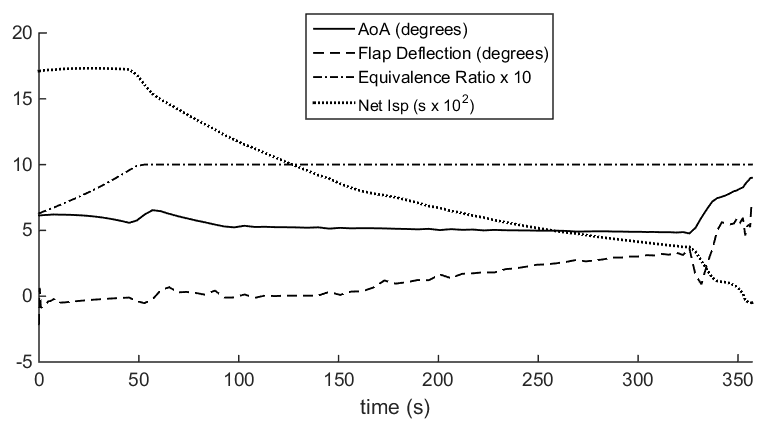
\includegraphics[width=.6\linewidth]{figures/5_Ascent/qlimited-Vehicle}
	\caption{Vehicle performance data for 50kpa dynamic pressure limited trajectory. Note: Flap deflection is positive down.}
	\label{fig:qlimited vehicle}
\end{figure}



LODESTAR is configured to optimise the total payload mass to orbit.
A maximum dynamic pressure limit of 50kPa is applied to the optimisation process to allow direct comparison with the constant $q$ trajectory and so that an equivalent vehicle can be used.   


The optimal trajectory shape for a $q=$50kPa limited, maximum payload to orbit trajectory is shown in Figures \ref{fig:qlimited}, \ref{fig:qlimited aero} and \ref{fig:qlimited vehicle} with key results summarised in Table \ref{table:Summary}. 
The equivalence ratio of the engine is less than 1 until 52.77s, causing the SPARTAN to fly under 50kPa in this region (to a minimum of 40.8kPa) in order to raise equivalence ratio by flying in a higher temperature region. This increase in equivalence ratio results in a corresponding increase in net specific impulse.
After the equivalence ratio increases to 1, the trajectory follows a constant dynamic pressure path at 50kPa until 331.7s at which point a pull-up manoeuvre is performed, gaining altitude until rocket stage release at \FlightTimeFiftykPa s flight time. 
This trajectory is able to deliver \PayloadToOrbitFiftykPa kg of payload to heliocentric orbit, an increase of \PayloadImprovement\ over the constant dynamic pressure result with minimum pull-up. The point at which the pull-up manoeuvre begins is the optimisation result that takes into account the best combination of velocity, altitude and release angle for scramjet stage performance and the release of the rocket stage. This pull-up indicates the region at which increasing altitude and release angle becomes more important than extracting maximum thrust from the scramjet (which is attained at high $q$ and low flight angle at an equivalence ratio of 1).
Flight in a lower dynamic pressure environment results in less thrust output from the scramjet engines, as well as an increase in angle of attack and flap deflection angle to compensate for the additional lift required. Due to this, less overall acceleration is obtained compared to the constant dynamic pressure result with minimum pull-up. Separation occurs at a velocity of \SeparationvFiftykPa m/s, a decrease of 24m/s. However, at the same time separation altitude increases by 1.32km to \SeparationAltFiftykPa km, resulting in a decrease in separation dynamic pressure to \SeparationqFiftykPa kPa. 

The larger scramjet stage pull-up assists the rocket in manoeuvring to exoatmospheric altitude by increasing the altitude and angle at separation by virtue of the increased L/D ratio and manoeuvrability of the scramjet vehicle. Even a small increase in release angle, to the optimal angle of \SeparationAngleFiftykPa~$^\circ$, significantly reduces the turning that is required by the rocket as evident from comparing Fig \ref{fig:ThirdStageConstQ} and \ref{fig:ThirdStage50kPa}. Further benefits are the reduced time that the rocket must spend in a high dynamic pressure environment, and a decrease in the maximum dynamic pressure that the rocket stage experiences by \qDecrease, as shown in Table \ref{table:Summary}. This allows the structural mass and heat shielding, necessary to achieve exoatmospheric flight, to be decreased, enabling higher payload to orbit. 


Compared to studies considering vehicles with a scramjet-rocket transition within a single stage\cite{Lu1993}\cite{Trefny1999}, the maximum payload to orbit trajectory of the multi-stage system shows a scramjet-rocket transition point at much lower altitudes.
This lower transition point is a consequence of the stage separation creating an energy trade-off, which does not occur in a single stage vehicle. Single-stage vehicles must necessarily transport all components to exoatmosphere, and so utilise the scramjet engines until higher altitude to take advantage of their high efficiency. A multi-stage vehicle is able to separate the scramjet stage. 
This separation occurs when the performance benefits provided by the superior aerodynamics and engine efficiency of the scramjet stage are offset by the energy required to lift the extra mass to higher altitude. The beneficial ability
to separate the scramjet stage results in a lower altitude scramjet-rocket transition point, when compared to single
stage vehicle designs.

\subsubsection{Dynamic Pressure Sensitivity}\label{subsection:qvariation}
\begin{figure}[ht]
	\centering
	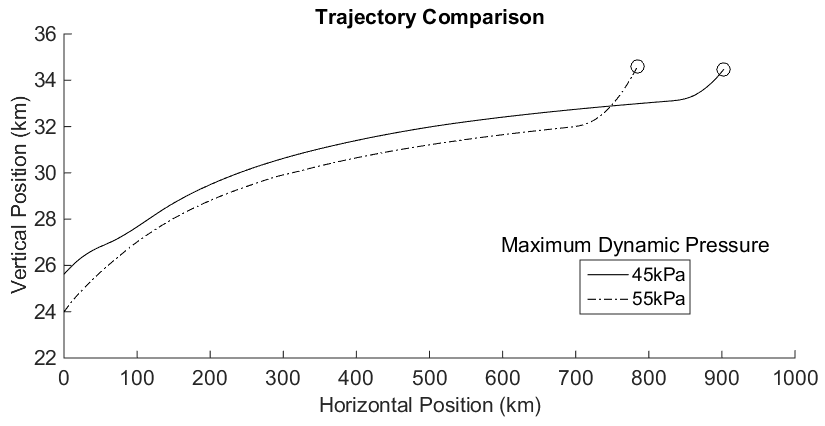
\includegraphics[width=.7\linewidth]{figures/5_Ascent/Multipleq}
	\caption{Comparison of 45kPa / 55kpa dynamic pressure limited trajectory paths for maximum payload to orbit.}
	\label{fig:multipleq}
\end{figure}
\begin{figure}[ht]
	\centering
	
	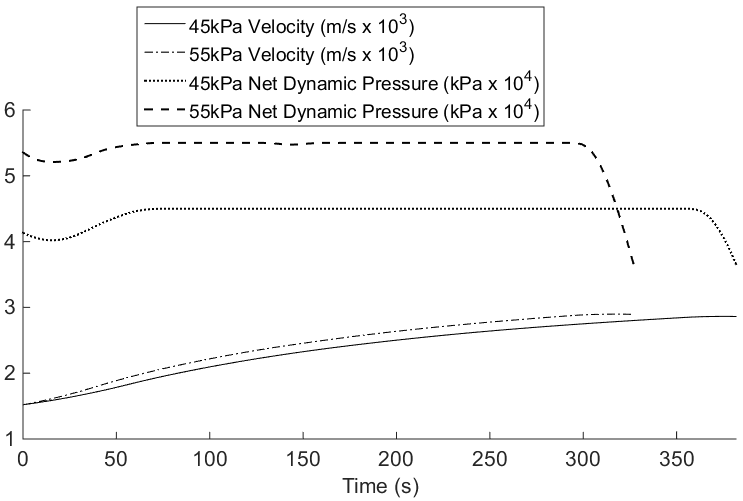
\includegraphics[width=.6\linewidth]{figures/5_Ascent/MultipleqAero}
	\caption{Comparison of trajectory data for 45kPa / 55kpa dynamic pressure limited trajectories.}
	\label{fig:multipleq aero}
\end{figure}
\begin{figure}[ht]
	\centering
	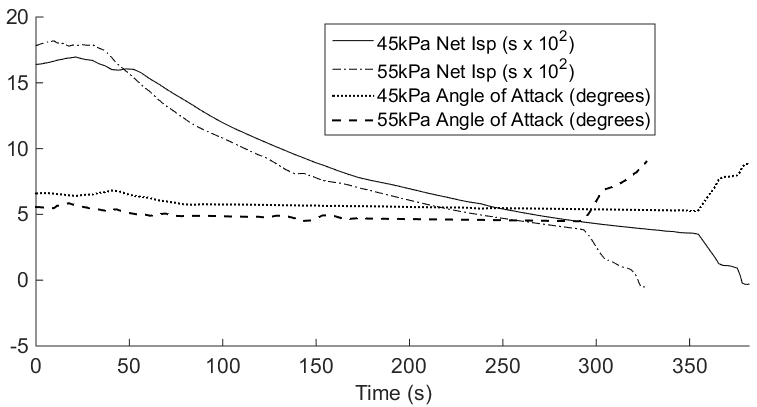
\includegraphics[width=.6\linewidth]{figures/5_Ascent/Multipleq-Vehicle}
	\caption{Comparison of vehicle performance data for 45kPa / 55kpa dynamic pressure limited trajectories.}
	\label{fig:multipleq vehicle}
\end{figure}
To investigate the sensitivity of the vehicle to changes in $q_{max}$, the maximum dynamic pressure is varied to 45kPa and 55kPa and the flight trajectory optimised, with results shown in Figures \ref{fig:multipleq}, \ref{fig:multipleq aero} and \ref{fig:multipleq vehicle} and summarised in Table \ref{table:Summary}.
The $\pm10\%$ variation in maximum dynamic pressure has very little effect on the payload mass delivered to heliocentric orbit.  Varying the maximum dynamic pressure by $\pm$5kPa from 50kPa causes a variation of only  \qVariationPluskg (\qVariationPlus) or \qVariationMinuskg (\qVariationMinus) in payload to orbit.  
Separation altitudes of \SeparationAltFortyFivekPa km and \SeparationAltFiftyFivekPa km are reached  for 45kPa and 55kPa limited cases respectively, with separation velocities of \SeparationvFortyFivekPa m/s and \SeparationvFiftyFivekPa m/s. The 45kPa limited case flies for \FlightTimeFortyFivekPa s, significantly longer than the 55kPa case which flies for \FlightTimeFiftyFivekPa s.
Both trajectories pull-up to similar altitudes, with relatively small variation in separation velocity \vVariationMinus m/s or \vVariationPlus m/s).
This small variation in velocity is despite the increase in air density and decrease in angle of attack required for flight at 55kPa dynamic pressure, both of which increase the mass flow into the engine. Although the thrust output of the REST engines increases with dynamic pressure, so does the drag on the vehicle, and the net increase in performance is small. 


Only a small variation in optimal payload mass is observed, without modification of vehicle design to account for the dynamic pressure limit. This indicates that designing and operating a vehicle at lower dynamic pressures may be preferable. Flying at a lower maximum dynamic pressure allows reduction of the structural weight and heat shielding of the vehicle. However, as the 45kPa limited case has a higher first-second stage separation altitude, a larger first stage fuel mass is required, though this increase in fuel mass is small. Between \FirstStageAltFortyFive km  and \FirstStageAltFiftyFive km (45kPa and 55kPa optimal start points) there is only a \FirstStagemincrease \% variation in the fuel mass required. This small variation in first stage fuel consumption would easily be offset by a decrease in second stage structural mass. 


\subsubsection{Drag Sensitivity Analysis}\label{subsection:dragvariation}
\begin{figure}[ht]
	\centering
	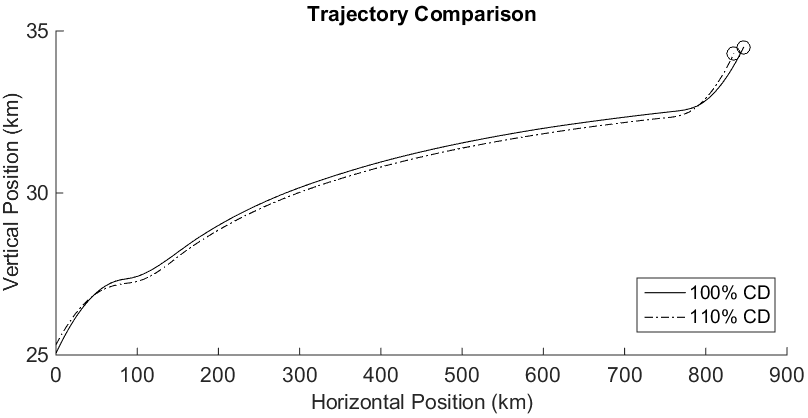
\includegraphics[width=.7\linewidth]{figures/5_Ascent/DragComparisonTraj}
	\caption{Comparison of trajectory paths for 100\% and 110\% drag cases for a 50kPa dynamic pressure limited maximum payload trajectory.}
	\label{fig:DragCompTraj}
\end{figure}

\begin{figure}[ht]
	\centering
	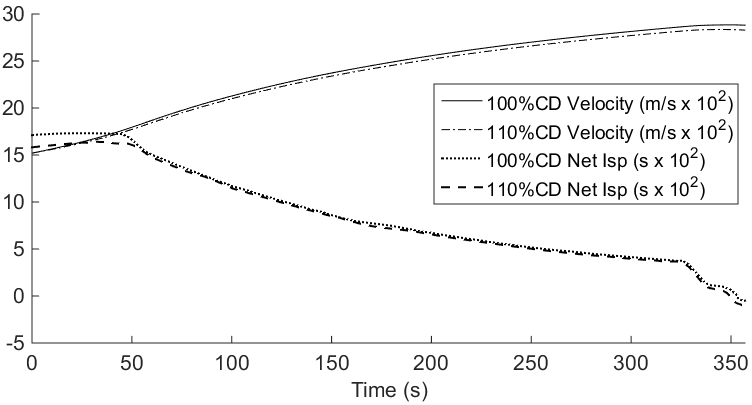
\includegraphics[width=.6\linewidth]{figures/5_Ascent/DragComparisonOther}
	\caption{Comparison of $v$ and $I_{sp_{net}}$ for 100\% and 110\% drag cases for a 50kPa dynamic pressure limited maximum payload trajectory.}
	\label{fig:DragCompOther}
\end{figure}

To investigate the effect of vehicle design and uncertainty in aerodynamic performance on the optimal trajectory the drag on the vehicle is increased by 10\%, and an optimised trajectory calculated with dynamic pressure limited to 50kpa. Selected results are compared to the 100\% drag result in Figures \ref{fig:DragCompTraj} and \ref{fig:DragCompOther}. 
These results show that when drag is increased (ie. L/D is decreased) the optimal trajectory shape is similar to the base-line case, though the high drag second stage follows a slightly slower and hence lower flight path, with a lower stage transition point. The similar flight path shape of the high drag case suggests that sacrificing velocity to increase separation altitude in a pull-up manoeuvre is optimal for multiple vehicle designs. Although the lower transition point indicates that the rocket is favoured at an earlier point in the climb manoeuvre, due to the decreased aerodynamic efficiency of the scramjet vehicle. 
The net result is  a lower payload-to-orbit of \PayloadToOrbitHighDrag kg (a decrease of 4.8\%). 




\subsection{Third Stage Evaluation}

Third stage trajectories for release angles of \SeparationAngleConstq $^\circ$ and \SeparationAngleFiftykPa $^\circ$ are shown in Figures \ref{fig:ThirdStageConstQ} and \ref{fig:ThirdStage50kPa}. 
These trajectories correspond to third stage release points at the end of a constant dynamic pressure trajectory with minimum pull-up (as shown in Section \ref{subsection:Fixed}) and an optimised 50kPa limited trajectory  (as shown in Section \ref{subsection:50kPalimit}). 
These third stage trajectories show a pull-up to high altitude before the circularisation burn is performed. 

The third stage released at 1.5$^\circ$, shown in Figure \ref{fig:ThirdStageConstQ}, is limited by the maximum thrust vector angle for the first 47s of flight. This places significant limitations on the maximum allowable angle of attack. This angle of attack limitation reduces the lift of the rocket, causing it to spend a large amount of time at low altitude, in a high drag environment. The angle of attack increases gradually to a maximum of 17.6$^\circ$ at 66s before decreasing until burnout at 140s. 

The release of the third stage rocket from an optimised scramjet trajectory is shown in Figure \ref{fig:ThirdStage50kPa}. Release at a higher, more optimal angle, mitigates the effects of the thrust vector angle limitation, so that the thrust vector limit is only reached during the first 10s flight time. After this, the angle of attack is limited by the maximum allowable normal force rather than the thrust vector limit, resulting in a higher maximum angle of attack. The rocket increases flight path angle and gains altitude rapidly, resulting in less time spent in a high drag environment, and a larger payload to orbit.  The angle of attack is increased gradually to 18.14$^\circ$ at 48s, before decreasing until burnout at 138s.

\begin{figure}[ht]
	\centering
	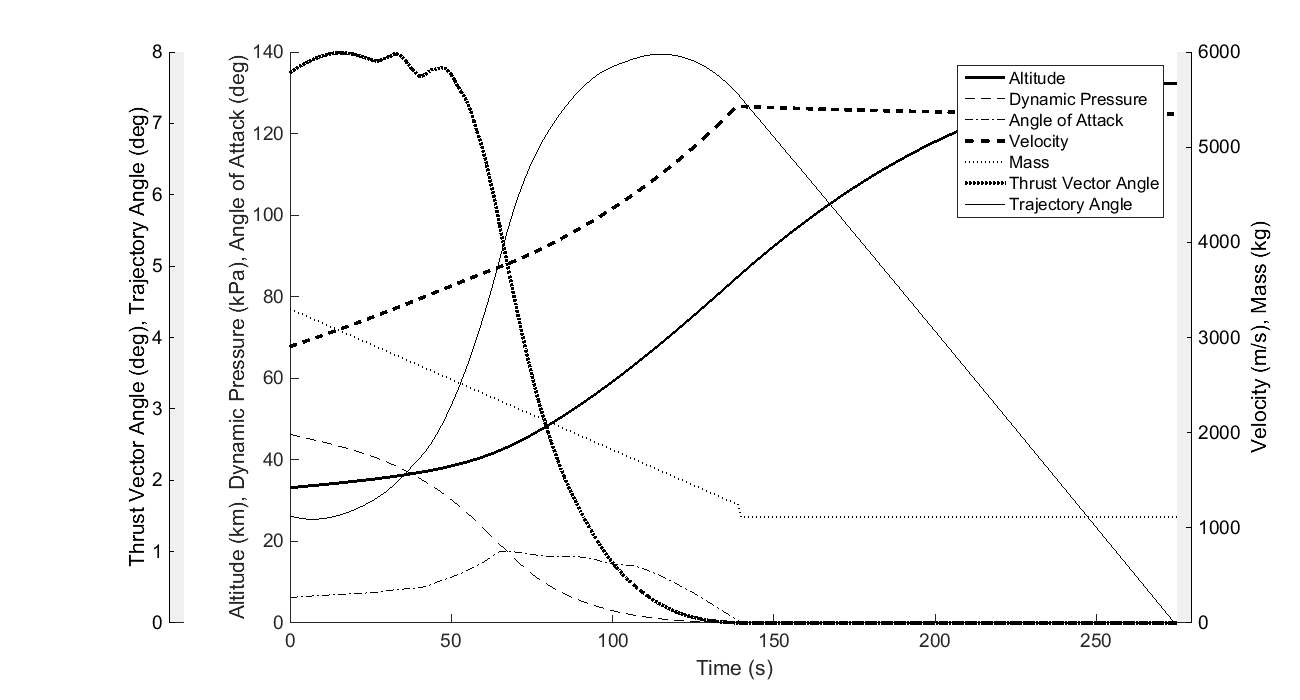
\includegraphics[width=0.8\linewidth]{figures/5_Ascent/ThirdStageConstQ}
	\caption{Third stage rocket trajectory simulated from the end of the 50kPa constant dynamic pressure SPARTAN trajectory, released at an angle of \SeparationAngleConstq $^\circ$, velocity of \SeparationvConstq m/s, and altitude of \SeparationAltConstq km.}
	\label{fig:ThirdStageConstQ}
\end{figure}
\begin{figure}[ht]
	
	\centering
	\includegraphics[width=0.8\linewidth]{figures/5_Ascent/ThirdStage50kpaConstrained}
	\caption{Third stage rocket trajectory simulated from the end of the 50kPa dynamic pressure limited maximum payload SPARTAN trajectory, released at an angle of \SeparationAngleFiftykPa $^\circ$, velocity of \SeparationvFiftykPa m/s, and altitude of \SeparationAltFiftykPa km.}
	\label{fig:ThirdStage50kPa}
\end{figure}